\section{Hoppers!}


\frame{
    \frametitle{\secname}
    \begin{figure}
        \centering
        
\includegraphics[width=0.65\linewidth]{slides//cryptids/beaverdam.png}
    \end{figure}
}

\section{A Brief Introduction to Busy Beavers}



\frame{
    \frametitle{\secname}
      \begin{wideitemize}
        \item<1-> Turing Machine (TM): A finite state machine reading and writing to an infinite tape of symbols. Basically simulates modern computers.
        \item<2-> TM halts if it reaches a halting state.\textbf{Halting problem} is well known to be undecidable. 
      \end{wideitemize}
      \begin{center}
          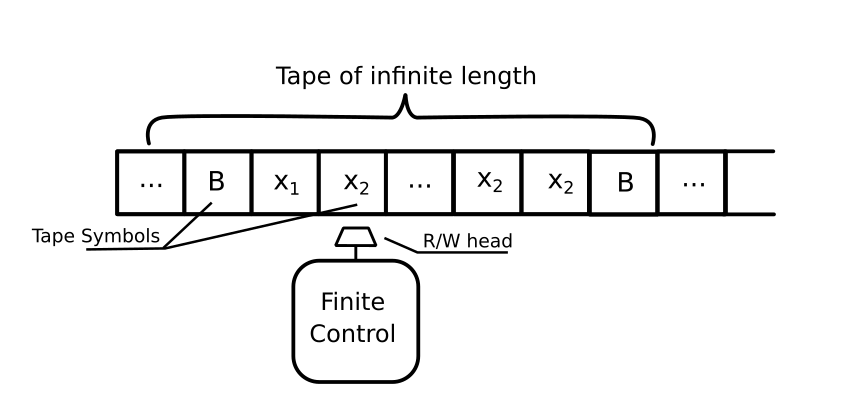
\includegraphics[width=0.55\linewidth]{slides/cryptids/turingmachine_tape.png}
      \end{center}
}

\frame{
    \frametitle{\secname}
  \begin{columns}
      \column{0.6\textwidth}
      \begin{wideitemize}
        \item<1-> What if we only look at TMs that \textbf{will halt}?  How many steps does it take for all halting TMs to finish their computation? \\

        \item<2-> For a halting TM $\mathcal{M}$ with $n$ states that can write $\{0,1\}$, $\mathcal{M}$ is an $n$-state Busy Beaver if it runs for the maximum number of steps across all halting $n$-state TMs. \\

        \item<3-> $S(n) = $ that maximum number of steps
      \end{wideitemize}
      \column{0.4\textwidth}
      \begin{center}
          
\includegraphics[width=0.9\linewidth]{slides/cryptids/hoppers.png}
      \end{center}
  \end{columns}
}

\frame{
    \frametitle{\secname}
  \begin{wideitemize}
    \item<1-> How do we compute $S(n)$?\\

    \item<2-> You don't. $S(n)$ is an non-computable function\footnote{Radó, Tibor (May 1962). "On non-computable functions" (PDF). Bell System Technical Journal. 41 (3): 877–884. doi:10.1002/j.1538-7305.1962.tb00480.x}.

    \item<3-> But we can still try to figure out what $S(n)$ is! \\

    \item<4-> What do you think comes next in the following sequence?    
    \begin{tabular}{|c||c|c|c|c|c|c|}
        \hline
        $n$ & $2$ & $3$ & $4$ & $5$ & $6$  \\
        \hline
        $S(n)$ & $6$ & $21$ & $107$ & $47176870$ & ??? \\
        \hline
    \end{tabular}
  \end{wideitemize}
}

\section{The Difficulty of Computing \texorpdfstring{$S(n)$}{S(n)}}

\frame{
    \frametitle{\secname}
    \begin{wideitemize}
        \item<1-> In order to show that $S(n) \leq X$, one must show that every TM with $n$ states either 
        \begin{itemize}
        \item Halts in at most $X$ steps, or 
        \item Does not halt.
        \end{itemize}
        
        \item<2-> What if we construct TMs that halt if and only if some other problem is true?
        
        \item<2-> If an $n$-state TM $\mathcal{M}$ halts if and only if some conjecture $P$ is true, then proving $S(n) = X$ means that $\mathcal{M}$ either halts in $X$ steps or never halts.

    \end{wideitemize}
}



\section{Cryptids}

\frame{
    \frametitle{\secname}
  \begin{columns}
      \column{0.6\textwidth}
      \begin{wideitemize}
        \item Coined by Shawn Ligocki in 2023.
        
        A \textbf{cryptid} is a TM that halts if and only if some hard conjecture is true/false.

        \item Cryptids exist for many hard mathematical conjectures
        \begin{itemize}
            \item Collatz Conjecture  
            \item Goldbach Conjecture 
            \item Riemann Hypothesis
            \item Consistency of PA and ZF set theory
        \end{itemize}
      \end{wideitemize}
      \column{0.4\textwidth}
      \begin{center}
      
\includegraphics[width=0.8\linewidth]{slides/cryptids/lovecraftian_beaver.png}
      
      {\tiny 
      \href{https://wiki.bbchallenge.org/wiki/File:Lovecraft_beaver.png}{Made by Lauren (2025), from Busy Beaver Challenge Wiki}
      }
      
      
      \end{center}
  \end{columns}
}

